We measure the expressibility of our VQC ansatz following Sim et al.~\cite{sim2019expressibility}.
The expressibility metric is defined as the KL divergence between the
fidelity distribution of random circuit parameter pairs and the Haar-random
reference:
\begin{equation}
  \mathrm{Expr} = \KL\!\bigl(P_{\mathrm{VQC}}(F)\,\|\,P_{\mathrm{Haar}}(F)\bigr),
\end{equation}
where $F = |\langle\psi(\theta_1)|\psi(\theta_2)\rangle|^2$ is the state
fidelity.  Lower values indicate more uniform coverage of the Hilbert space.

We compute this metric on $n=3$ qubits using 10{,}000 random parameter
samples with \texttt{StronglyEntanglingLayers} at depths $d \in \{1,\dots,5\}$,
compared against a classical random linear projection baseline.

\begin{table}[h]
\centering
\caption{Expressibility (KL divergence from Haar) for 3-qubit VQC at various depths vs.\ classical linear projection.}
\label{tab:expressibility}
\small
\begin{tabular}{lr}
\toprule
Model & KL Divergence \\
\midrule
VQC depth=1      & 0.2021 \\
VQC depth=2      & 0.0048 \\
VQC depth=3      & 0.0027 \\
VQC depth=4      & 0.0027 \\
VQC depth=5      & 0.0027 \\
Linear proj.     & 1.9098 \\
\bottomrule
\end{tabular}
\end{table}

Expressibility saturates at depth $\approx 3$, with diminishing returns
beyond that.  The classical linear projection baseline is roughly three
orders of magnitude less expressive, confirming that even shallow VQC
layers access a significantly richer region of Hilbert space.
Figure~\ref{fig:expressibility} shows the fidelity distributions and
KL divergence comparison.

\begin{figure}[h]
  \centering
  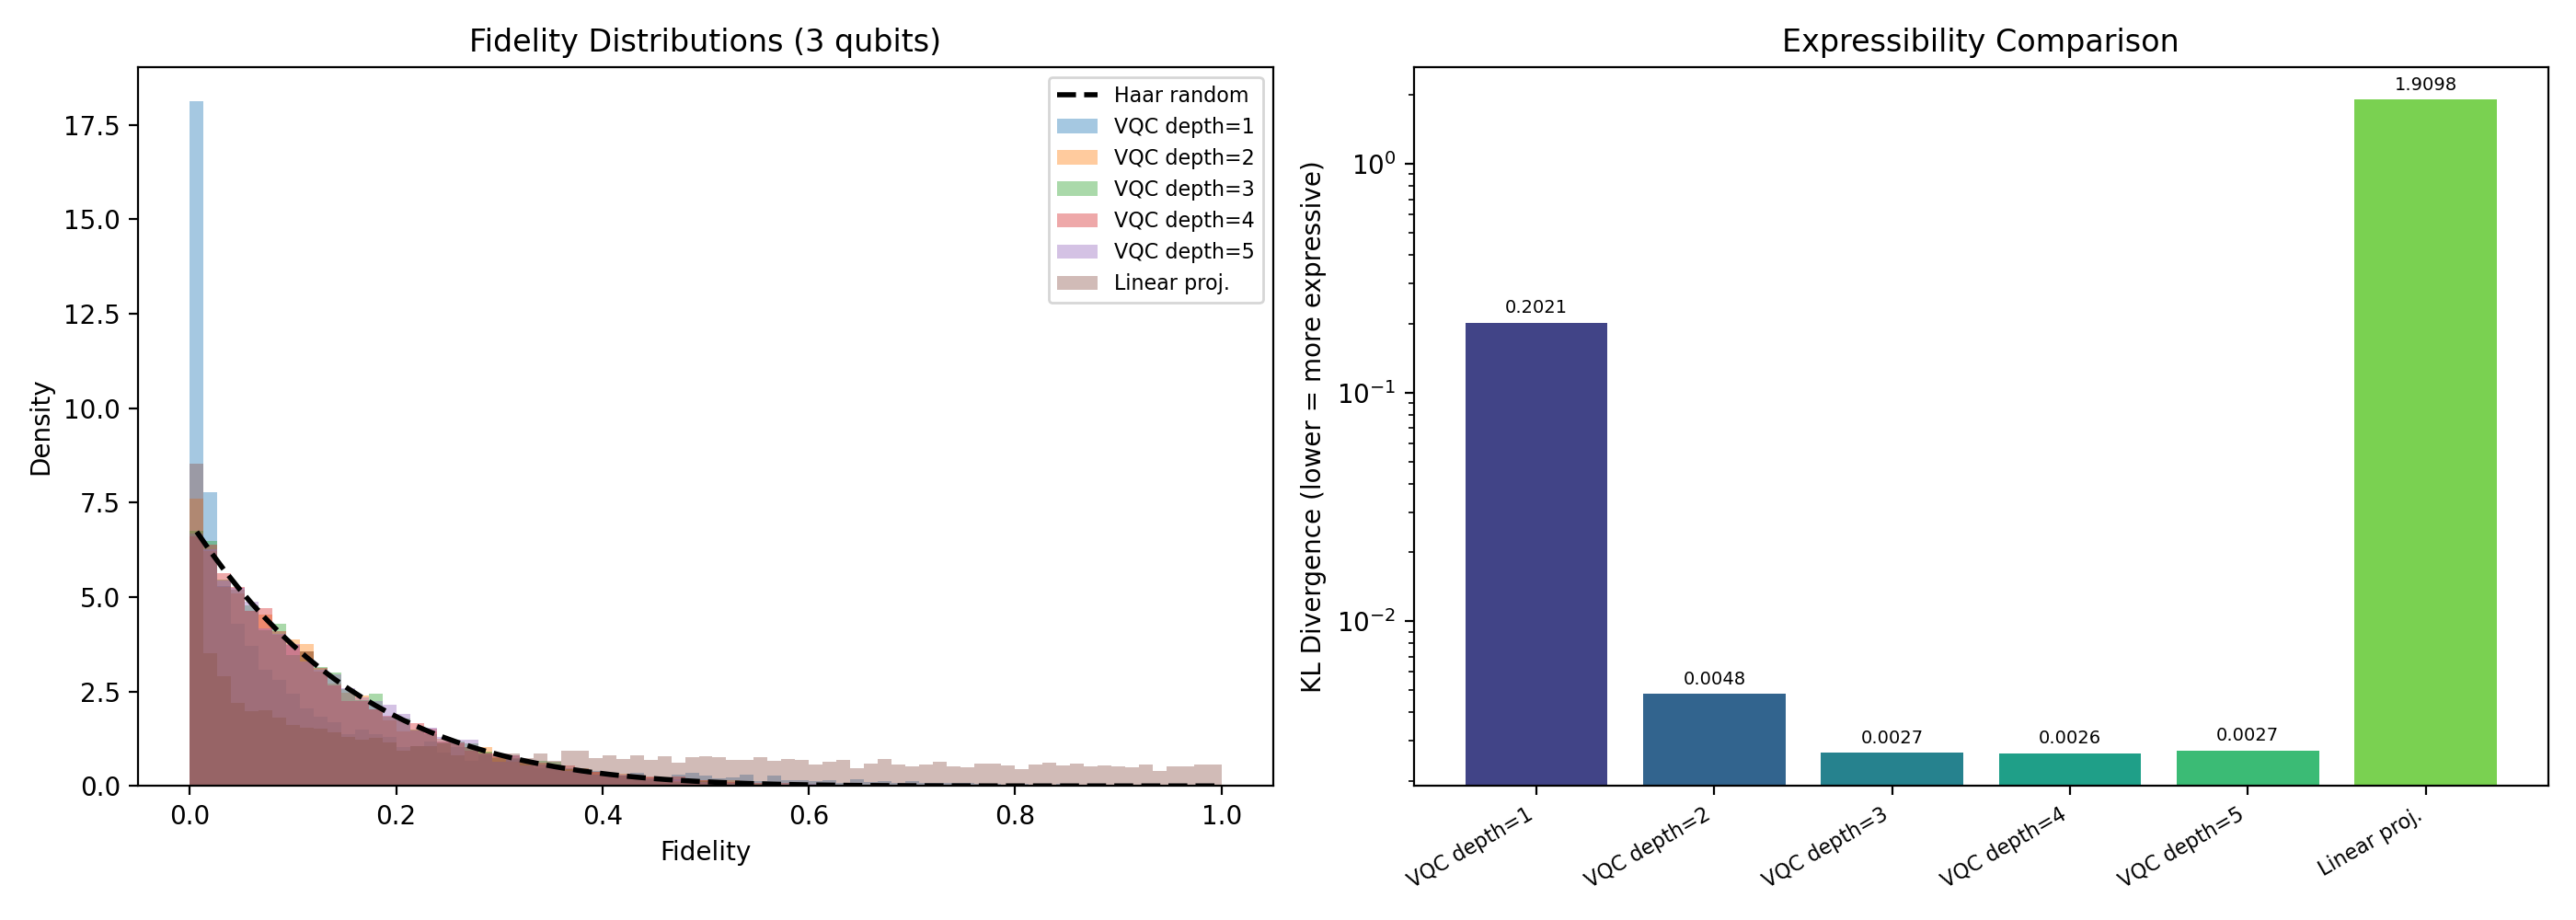
\includegraphics[width=\columnwidth]{figures/expressibility_results.png}
  \caption{Left: fidelity distributions for VQC at various depths vs.\
  Haar-random reference (dashed). Right: KL divergence (log scale).}
  \label{fig:expressibility}
\end{figure}
